
\chapter{The ``software crisis'' and encapsulation}

\index{object-oriented}
This book is going to dive deeply into a huge pile of nuts and bolts. But
before we take the leap into particulars, it's important to stand briefly at
the precipice and understand why we're jumping. What does ``object-oriented''
mean? What problem was it intended to solve? When was it invented and why?

\section{Ancient history}

\index{software crisis}
\index{1970@the 1970's}
A long time ago, in our own galaxy, a situation emerged which has been labeled
\textbf{the software crisis}. This crisis didn't happen at an instant in time;
it was a set of disagreeable circumstances which gradually evolved until it
became unbearable. The crisis is usually dated somewhere in the 1970's. This
was just as the high-tech computing industry was really starting to heat up,
on its way to permanently changing the lives of almost everyone on the planet.

Now ``crisis'' is an alarming word, designed to get your attention. It's worth
asking what all the hubbub was about. The immediate symptom may not strike you
as a three-alarm fire: it was simply that software projects were tending to
overrun their schedules.

The '70's were not a very plug-and-play era, since standards had not yet
evolved to facilitate intercompatibilities between devices or programs. So the
focus was often on building complete systems from the ground up. Engineering
teams would plan releases of key product lines that involved numerous
components, such as system architecture, hardware design and integration, data
collection and organization, system and network configuration, and software
development at both the operating system and the end user levels.

\index{software@``software''}
\index{hardware}
What managers discovered was that the \textit{software} components of projects
were consistently coming in late and over-budget. Sometimes, they didn't get
finished at all. When they did, they were buggy and brittle. And they were
especially vulnerable to requirements changes: if circumstances were
discovered during the project that required a change in the way the software
needed to work, the software team was often strikingly unable to adapt to
this. They could be set back weeks or months to implement even a modest
change.

This astonished everyone at the time. After all, ``\textit{soft}ware'' -- a
pun on ``hardware'' -- was a term intended to convey the flexible, malleable
nature of computer programs as contrasted with physical devices. Software was
supposed to be easy to write and easy to change. That was the point. You
didn't need complex manufacturing processes: you needed a desktop computer and
a text editor. And you (seemingly) didn't face challenges of scale the way you
did with hardware: you could run out of room to put logic circuits on a chip
or a motherboard, but there was no limit to the size of a text file. 

So building complex stuff quickly, and turning on a dime when necessary, ought
to be easy to do in software. Right?

\subsection{Quantifying the crisis}

I've never seen any hard data quantifying the budget overruns and delays that
software projects faced in the 1970's. It's possible to sketch it
conceptually, though. Take a look at Figure~\ref{fig:complexityCurve}. This is
my attempt to show the main dynamic at work.

\begin{figure}[ht]
\centering
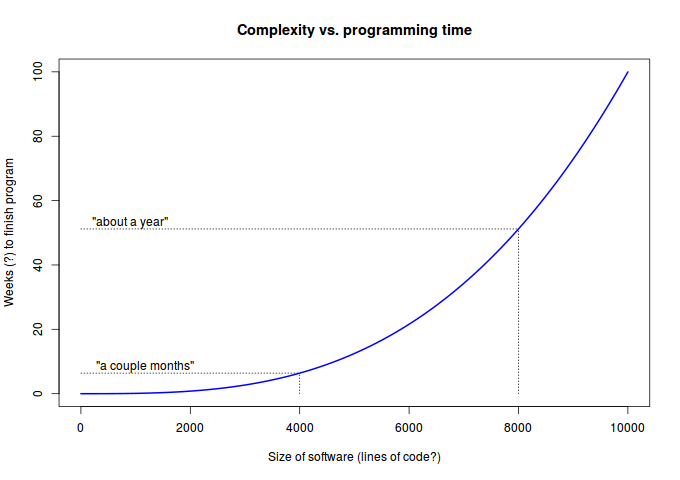
\includegraphics[width=0.9\textwidth]{complexityCurve.png}
\caption{The software crisis quantified: how long it took to complete a
program of various sizes. (Conceptual.)}
\label{fig:complexityCurve}
\end{figure}

\index{complexity}
\index{LOC (lines of code)}
\index{KLOC (thousands of lines of code)}
On the $x$-axis is some measure of the \textit{complexity} of a proposed
computer program. Now complexity is devilishly difficult to quantify -- League
of Legends is more complex than Angry Birds, but by how much? Twice as
complex? Ten times? A hundred times? I'll have a better answer to that in a
few paragraphs, but for now, as a proxy we'll just use the \textit{size} of
the program, measured in \textbf{lines of code}\footnote{I know what you're
thinking, and you're right. Not all lines of code are equally complex. Some of
them are just variable assignments, whereas others are parts of complicated
loops or function calls. Heck, some are just comments. Heck, some are actually
\textit{blank}. While all true, this analysis is conceptual anyway, and we can
surely say that raw program length is at least \textit{somewhat} related to
complexity. Show me a real-life ten-line program that's actually more complex
than a real-life ten-thousand-line program and I'll change my mind.} (``LOC''
or ``KLOC.''\footnote{``Lines of code'' is sometimes abbreviated ``LOC.'' Even
more common is the abbreviation ``KLOC'' for ``thousands of lines of code.''}

On the $y$-axis is the corresponding amount of time it would take a
programming team of a certain size to design, build (code), and test the
program.\footnote{Note carefully that this has nothing to do with how long the
code takes to \textit{run}. We're talking about programmer-time here, not
CPU-time.} As with the $x$-axis, we're making all kinds of simplifying
assumptions here: we're not worrying about exactly how many developers
there are, how much experience they each have, what language they're writing
in, \textit{etc.} That's okay. The point of this exercise is simply to
recognize the nature of the curve, showing how these two fuzzy variables were
related in the '70's.

\index{project managers}
And a daunting curve it is, too. And very counterintuitive to project
managers. One would assume that if a 4,000-line program took the development
team a couple of months to release, an 8,000-line program would take about
twice that long. After all, it's twice as many lines, right?

The reality was not even close. A program with twice as many lines could
easily take \textit{four} times as long to build...or six, or ten, or twenty
times. Worse, the programs that were built were also very hard to
\textit{change}. Take a large enough program and try to add a feature, fix a
bug, or support a new data format, and you inevitably broke something else
while making the change. Then you fixed what you broke, but \textit{d'oh!!}
broke something else by doing so, \textit{etc.}

\index{hardware}
\index{software@``software''}
It was miserable, especially because advances in other areas (like hardware)
were making exciting technologies possible for the first time. Everyone was
rarin' to go, yet unexpectedly the software (supposedly the easy part) was
gumming up the works.

\index{maximum complexity@``maximum complexity''}
For a time, it almost seemed as if the human race had uncovered some built-in
limitation of the universe, like the speed of light. This hypothetical
constant might have been called ``maximum complexity,'' meaning the greatest
amount of sophistication one could build in to a single logical creation. That
curve in Figure~\ref{fig:complexityCurve} starts to go up fast. Maybe, people
depressingly thought, a functioning 200,000-line program isn't even
\textit{possible} to create? That threatened to put a damper on a lot of
expectations.

\section{Software and complexity}

\index{complexity}
\index{code chunks!code ``chunks''}
\index{dependency!between code chunks}
Let's consider a different way to measure a program's complexity than simply
counting the lines of code. Instead, let's quantify its number of
\textit{dependencies}.

A \textbf{dependency} between two chunks of software (be they individual lines
of code, constructs like loops or if/else chains, functions, or something even
bigger) means that \textit{if one of them changes, the other may possibly be
affected.}

\index{compute\_sales\_tax@\texttt{compute\_sales\_tax()}}
For instance, suppose I define a function \texttt{compute\_sales\_tax()} to
take one argument: the price of an item. It will return the sales tax on that
item as a simple percentage. We'll call that ``code chunk A.'' Now suppose
that I call the function in ``code chunk B'' as follows:

\begin{Verbatim}[fontsize=\small,samepage=true,frame=single]
   // In code chunk B...
   double item_price = 24.99;
   double total_price = item_price + compute_sales_tax(item_price);
\end{Verbatim}

We say that code chunk B has a dependency on A. If we were to change A to
require a second parameter (perhaps the state the customer lives in, since
different states have different laws about whether and how to collect sales
tax), that's great and all, \textit{but B immediately breaks} unless we change
it as well.

\index{dependency!syntactic}
\index{dependency!logical}
This example is a syntactic dependency: the compiler will fail when trying to
compile code chunk B because its parameter list is wrong (\textit{i.e.},
doesn't match A's). In general, though, not all dependencies are merely
syntactic. There are also \textit{logical} dependencies, in which one chunk of
code depends on another's functionality working a certain way.

For example, suppose that we change \texttt{compute\_sales\_tax()} in a
different way: instead of returning the sales tax, we make it return the cost
of the item \textit{plus} the sales tax. If our tax rate is 5\%, then the
original version of \texttt{compute\_sales\_tax(24.99)} would return 1.25 (the
sales tax on the item), but our new version would return 26.24 (the item's
price with its sales tax added in).

This may seem like a good change, since it prevents code like that in chunk B
from having to add the item's price back in. However, if we don't change B in
tandem with A, \textit{B breaks again}. It's not a compilation error this
time, but a logic error: B's \texttt{total\_price} variable is now going to
contain 51.23 because we didn't keep the two chunks of code in sync.

\subsection{Dependencies == complexity}

\index{dependency}
\index{complexity}
\index{software crisis}
Now why do I bring all this up? Because it turns out that the \textit{length}
of a program was not the cause of the software crisis. Instead, it was
\textit{the number of dependencies} programs had. That turns out to be a
different, and more salient, measure of a program's complexity.

\begin{figure}[ht]
\centering
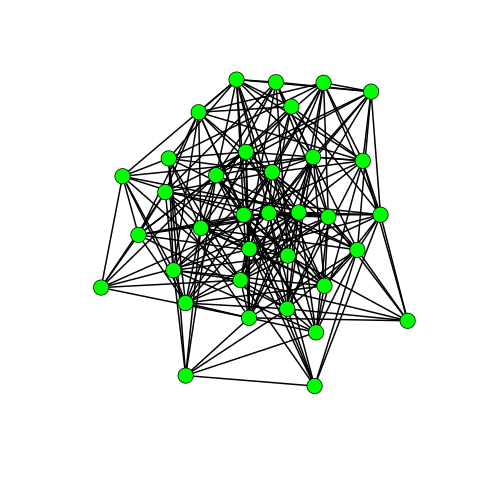
\includegraphics[width=0.45\textwidth]{highDependencies.png}
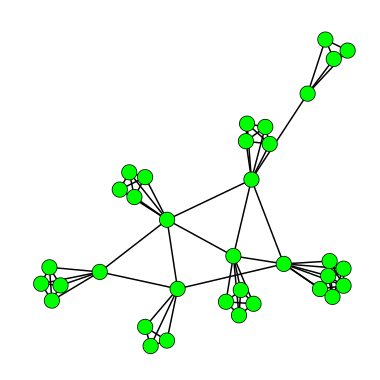
\includegraphics[width=0.45\textwidth]{lowDependencies.png}
\caption{Two programs, each with 35 code chunks. On the left, there are 230
dependencies. On the right, there are only 83.}
\label{fig:dependencies}
\end{figure}

\index{graph}
\index{vertex}
\index{node}
\index{edge}
\index{link}
Consider the two graphs\footnote{A \textbf{graph} in computer science terms is
a data structure that consists of \textbf{vertices} (or \textbf{nodes}) and
\textbf{edges} (or \textbf{links}) connecting them. They're often drawn with
circles and lines, as Figure~\ref{fig:dependencies} does.} in
Figure~\ref{fig:dependencies}. Imagine that each green circle represents one
chunk of code. Each line between circles represents a dependency: the two
chunks of code it connects rely on each other \textit{not} to change, because
if one of them changes, the other one might break.

\index{spaghetti code}
The kind of program illustrated by the left-hand graph sometimes goes by the
name \textbf{spaghetti code}. You can see why just by looking at it.
Essentially, every line of code potentially depends on everything else.

\index{modular}
\index{gatekeeper@``gatekeeper''}
By contrast, the right-hand graph depicts a \textbf{modular} program. It has
the same amount of functionality -- 35 green circles in each case -- but far
fewer dependencies between them (only about a third as many). Looking further,
you can see how most of the circles are ``hiding'' behind a gatekeeper circle
that connects to the main group. The majority of circles are shielded from the
morass of dependencies by living in an isolated world, and only communicating
with the rest of the program through their gatekeeper.

Now look back at the left-hand graph. Choose one of the circles at random, and
imagine that it represents a chunk of code you need to change (maybe there's a
bug in it you have to fix, or you need to extend it in some way). Think about
the repercussions of that task. Fixing the green circle is a job in itself,
but once you've done so, how can you be sure you didn't break something else?
There might be twenty other chunks of code that depend on the first one
staying the way it was in order to work correctly. Just identifying all of
them is an enormous task, to say nothing of verifying that they all still
work, and fixing the ones that don't. And oh, by the way: if you \textit{do}
end up having to fix another green circle because your first change caused a
ripple effect...that second change is going to cause the exact same problem.

The situation is obviously much easier with the right-hand program. Again,
choose a circle at random, and then ask yourself how onerous it is to change
it. If you choose one of the many circles that are ``hiding'' behind their
gatekeeper, the possible damage is minuscule: only three or four other circles
might be affected. If you have to change a gatekeeper, the news is worse, but
still far better than it was with the left-hand program. Just count how many
dependencies there are for even the most densely connected circle of the
modular program -- there ain't many.

\begin{figure}[ht]
\centering
\medskip
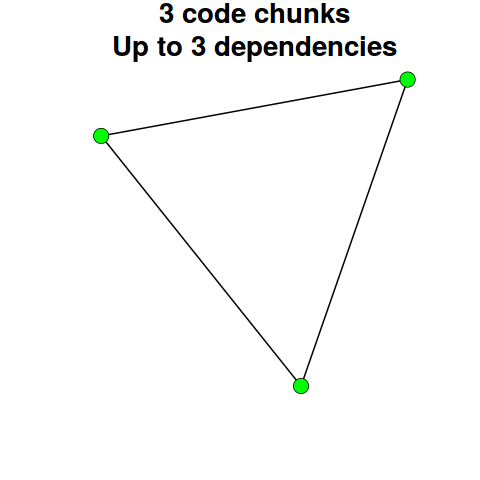
\includegraphics[width=0.31\textwidth]{dependencies3.png}
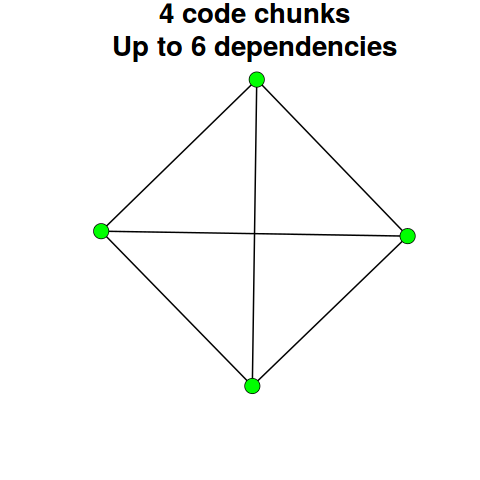
\includegraphics[width=0.31\textwidth]{dependencies4.png}
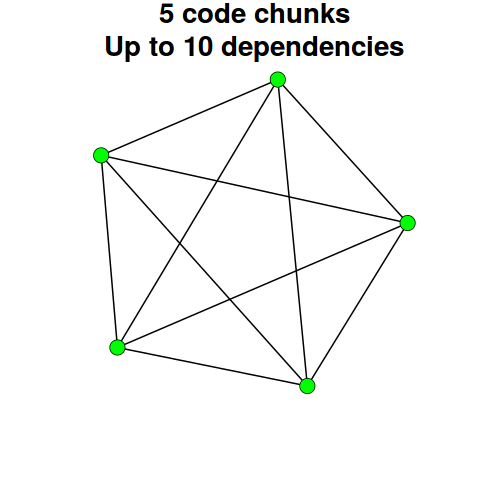
\includegraphics[width=0.31\textwidth]{dependencies5.png}

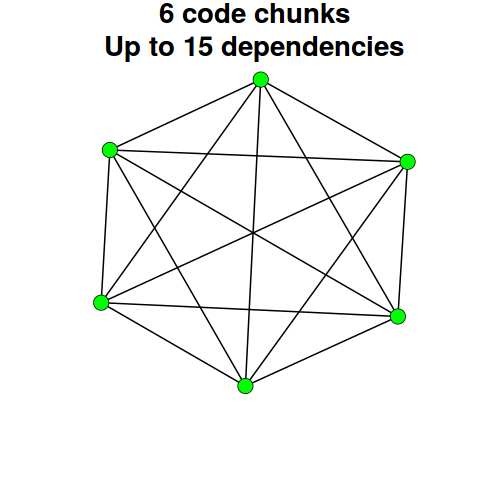
\includegraphics[width=0.31\textwidth]{dependencies6.png}
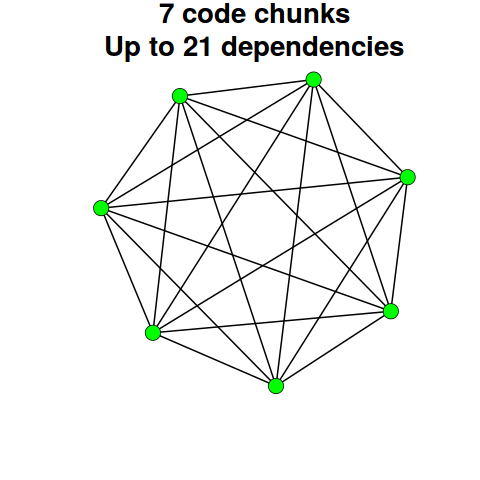
\includegraphics[width=0.31\textwidth]{dependencies7.png}
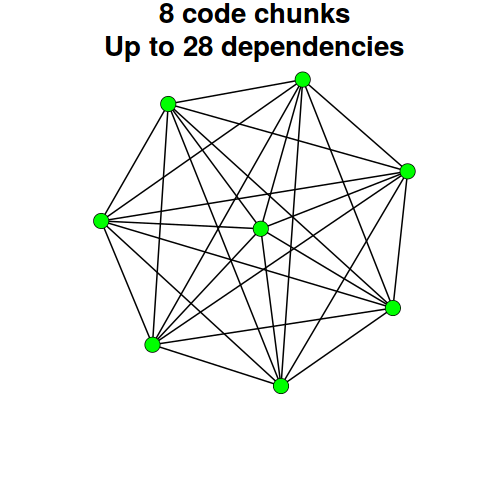
\includegraphics[width=0.31\textwidth]{dependencies8.png}
\caption{The maximum possible number of dependencies for programs of different
sizes.}
\label{fig:dependencyGrowth}
\medskip
\end{figure}

\index{superlinear}
\index{1970@the 1970's}
Figure~\ref{fig:dependencyGrowth} quantifies this further, and in fact finally
gives us the insight we need to understand the cause of the curve in
Figure~\ref{fig:complexityCurve} (on p.~\pageref{fig:complexityCurve}). If
you've taken a Discrete Math class, you may remember that the number of
possible edges in a graph goes up as the \textit{square} of the number of
vertices. (Specifically, a graph with $n$ vertices can have up to
$\frac{n(n-1)}{2}$, or about $\frac{n^2}{2}$, edges.) So doubling the
number of code chunks approximately \textit{quadruples} the number of possible
dependencies in the program. That explains why
Figure~\ref{fig:complexityCurve} was \textbf{superlinear} (\textit{i.e.},
increased faster than a straight line would have), and why everyone in the
'70's was underestimating how much time it would take to write and maintain
large programs.

\section{Encapsulation}
\index{dependency!between code chunks}

This, then, was the root cause of the software crisis. Larger programs, which
had more parts, inevitably produced too many interlocking dependencies between
their parts. Those dependencies were a killer: changing or adding any one part
threatened to break a dozen other parts. So a program with twice as many
features didn't take twice as long to construct; it took way more than twice
as long. And a program with ten times as many features looked plumb out of
reach.

\index{encapsulation}
And now finally, the punchline. The way the human race conquered the
dependency problem, and overcame the software crisis for good, was by means of
the single most important aspect of object-oriented programming:
\underline{\textbf{encapsulation}}. This feature gets far, far less press than
it should. It made possible all the complex software applications that the
world now relies on every day. It's one of the most important principles --
perhaps \textit{the} most important -- in all of computer science.

So what is encapsulation? In a word, it's an organizational principle that
permits many more green circles to be added to a program without also having
to add a zillion more pesky lines. It's a way to keep a program's dependencies
under control, so that as it grows larger, it doesn't also grow more brittle
and bug-prone.

Glance back at Figure~\ref{fig:dependencies} on p.~\pageref{fig:dependencies}.
Simply put, the right-hand program is employing encapsulation, and the
left-hand program is not. On the right, each of the little clusters of
tightly-knit green circles is ``encapsulated'' from the other clusters. That
isolates them safely behind a gatekeeper such that changing them will
\textit{not} trigger a chain reaction and require other changes.

\index{cohesive (highly)}
\index{coupled (loosely)}
In all the code we write, we want to strive for this. We want to make our
units of code highly \textbf{cohesive} yet loosely \textbf{coupled}. We want a
lot of small components (not a few large ones), and we want each component's
internal workings to be invisible to the outside world. It's the only way to
avoid the hell of spaghetti code.

\subsection{OOP's encapsulation solution: the \texttt{class}}

\index{class@\texttt{class}}
I've been using vague terms like ``chunks'' and ``units'' and ``components''
to refer to these bits of interacting software. The key innovation of OOP
(object-oriented programming) was a particular kind of ``unit,'' structured in
a particular way: the \textbf{class}. It changed the world.

\index{public interface}
\index{private implementation}
\index{gatekeeper@``gatekeeper''}
We'll be talking lots and lots about classes throughout this book. Every
single line of code we write, in fact, will be part of a class. For now, I
want you to imagine a class as being comprised of two parts: a \textbf{public
interface} and a \textbf{private implementation}. In terms of
Figure~\ref{fig:dependencies}, the public interface is the gatekeeper node
that connects each cluster to the whole, whereas the private implementation is
the other nodes in the cluster that hide behind the gatekeeper.

Another way of viewing this is Figure~\ref{fig:mostImportant}. The concentric
yellow circles represent a \textbf{class}, with its two components. To evoke a
biology metaphor, you can think of the public interface as the membrane of a
cell: nothing goes in or out of the cell body except through the membrane.

\begin{figure}[ht]
\centering
\includegraphics[width=0.8\textwidth]{mostImportant.pdf}
\caption{Encapsulation, visualized abstractly.}
\label{fig:mostImportant}
\end{figure}

Almost all the code for the class, including the variables it uses and the
bodies of its functions, are in the \textit{inner} circle, safely sequestered
away from the membrane. This means they are \textit{free to change} without
impacting any other part of the code that's using the class. The only things
in the outer circle are the function \textbf{signatures} (\textit{i.e.}, the
names, return types, and argument lists of the functions). This is the
information other parts of the code must know in order to make use of the
class.

The right-side of the diagram is my way of drawing a connection between
Figures ~\ref{fig:dependencies} and \ref{fig:mostImportant}. Each cluster of
green code chunks on that earlier diagram will form a \textbf{class}. The
``gatekeeper'' node through which all of the other code chunks must
communicate gets mapped to the public interface of the class, while all of the
other chunks are put in the private implementation.

\section{Features of OO}

The object-oriented revolution came about simply by taking what was formerly
spaghetti code, and learning how to organize it into encapsulated classes.
It'll take the whole book to completely unpack that, but for now let me give
you a glimpse of some of the features of this paradigm shift:

\begin{enumerate}
\itemsep.1em

\index{abstraction}
\index{function}
\index{procedural programming}
\item \textbf{A higher level of abstraction.} Before OOP, encapsulation was
already sort of a thing, since ordinary \textbf{functions} gave programmers a
way to group code chunks together into cohesive bits. In this old-style of
\textbf{procedural programming}, developers wrote code to compose and combine
these functions to achieve a larger purpose. The difference with OOP is that
the fundamental building block is no longer the function, but the class, which
is a bigger, richer, more sophisticated entity. It encompasses functions,
variables, and more besides. Being able to program ``at a higher level of
abstraction'' means you have larger, coarser-grained, more powerful pieces
with which to assemble your whole. It's like building a story out of whole
paragraphs instead of out of individual words or letters.

\index{noun}
\index{verb}
\item \textbf{Nouns, not verbs.} An old-school function is conceptually a
verb: it represents a command to \textit{do} something. As we'll see, a class
is conceptually a noun: it has the ability to \textit{be} something. Thus,
with OOP you don't think so much about what you want to \textit{execute} --
first do this, then that, then print the output -- as about what you want to
\textit{model} -- how can you best represent the important entities in your
system? OOP is about building a representation of a world, rather than giving
instructions.

\index{struct@\texttt{struct}}
\index{C++}
\item \textbf{Data and behavior \textit{together}.} Before the object-oriented
paradigm shift, programmers specified their data separately from the code that
operated on that data. They did this deliberately. In a C++ header file,
they'd write a number of \texttt{struct} definitions, each specifying an
assortment of related variable names and types. Then, in many separate source
files, they'd have lots of functions that used various of these structures.
The ``openness'' of all this -- any function, anywhere, could see and refer to
any field of any data structure -- was thought to be an advantage.

\index{sword}
\index{sweater}
After many years of painful discovery, it turned out this isn't the right way
to do it at all. Instead, you want the opposite. The data associated with a
particular type of entity (be it a friend request, a sweater, or a magic
sword) ought to be closely bound to the operations (\texttt{accept()},
\texttt{purchase()}, \texttt{wield()}) that make use of that data. This new
way of doing things is built in to the object-oriented \textbf{class}
construct: a class represents some type of entity, and it specifies both the
data needed to characterize instances of that entity and the operations that
can be performed on those instances. The two are defined right next to each
other and maintained in lock-step.

\index{code reuse}
\index{linked list}
\index{binary search tree}
\index{heapsort}
\item \textbf{Code reuse.} I'm old enough that I remember when ``code reuse''
was absolutely a pipe dream. People would think, ``okay, I need a linked list
(or a heapsort algorithm, or a binary search tree, or...), and surely zillions
of people have written this sort of thing before. However, it's just too hard
to find someone else's code, figure out how to use it, trust that it works,
and assimilate it into my program. So I'll just write it from scratch.''
Seriously: that's how the world worked. I wrote many programs in my early days
without using a single line of code from anyone else.

There were several reasons code reuse was hard, including poor documentation,
primitive search engines, and an overall lack of awareness in the software
community. But the \#1 reason was assuredly the absence of encapsulation. In
order to incorporate someone else's linked list (or whatever), you had to
locate portions of several different files, all of which were intertwined with
other stuff irrelevant to your purpose. You had to understand it enough to
gingerly insert it into multiple places in your own files, hoping it could
peacefully co-exist alongside your own code. The chances of this were low.

\index{library}
\index{encapsulation}
\index{dependency!between code chunks}
\index{Legos}
Nowadays, code reuse is absolutely the standard. If you're writing a program
these days, you should only write about 20\% of the code yourself; the rest
should come from standard libraries or other public sources. You can just grab
stuff and use it and be confident it'll work. Why is this easy? Because that
``stuff'' is encapsulated. It's modular, with no external dependencies. It's
all assembled coherently together in nice \& neat packages (called classes)
that are plug-and-playable. Writing a program is more like building with
Legos\textsuperscript{\textregistered} than it ever has been.


\end{enumerate}

\section*{Postlude}

This chapter was very abstract and qualitative. The rest of the book won't be
that way. But I felt it was important to lay some groundwork so that you would
appreciate what problem object-oriented programming was intended to solve, and
how through the miracle of encapsulation it did so. Thanks for making it
through.

%Doesn't it just come for free? No. Programmer's tendencies is always to
%un-encapsulate.

